\subsection{Input for the Campaign / Flight Requirements Plans}


\subsubsection{Dimensions and Mass}
\label{sec:dim-mass}

The data shown in Table \ref{tab:dim-mass-tab} below is based on the design presented in Section \ref{Mechanical_Design}. %The mass for the electronics is estimated to be 1.5 kg.

\begin{table}[h!]
\noindent\makebox[\columnwidth]{%
\scalebox{0.8}{
\begin{tabular}{c|c|c|c|c|}
\cline{2-5}
 & Telescope & Electronics & Gimbal & TOTAL  \\ \hline
\multicolumn{1}{|c|}{Experiment mass {[}kg{]}} & 5 & 1.5 & 5 & 13  \\ \hline
\multicolumn{1}{|c|}{Experiment dimensions {[}m{]}}& 0.651x0.222 &  & 0.1x0.1x0.1 &  & \\ \hline
\multicolumn{1}{|c|}{Experiment footprint area {[}$m^2${]}} & & 0.1 & & \\ \hline
\multicolumn{1}{|c|}{Experiment volume {[}$m^3${]}} & 0.0123 & 0.1 & & \\ \hline
\multicolumn{1}{|c|}{Experiment expected COG position} & \begin{tabular}[c]{@{}l@{}}$X=\ cm$\\ $Y=\ cm$\\ $Z=\ cm$ \end{tabular}  & \begin{tabular}[c]{@{}l@{}} $X=\ cm$\\ $Y=\ cm$\\  $Z=\ cm$ \end{tabular} &\begin{tabular}[c]{@{}l@{}} $X=\ cm$\\ $Y=\ cm$\\  $Z=\ cm$  \end{tabular} &\\ \hline
\end{tabular}}}
\caption{Experiment Summary Table.}
\label{tab:dim-mass-tab}
\end{table}


\subsubsection{Safety Risks}
Table \ref{tab:safrisk} contains the risks of all stages of the whole campaign and project.
\begin{table}[H]
    \centering
    \begin{tabular}{|m{0.2\textwidth}|m{0.35\textwidth}|m{0.35\textwidth}|}
    	\hline
    	\textbf{Risk} & \textbf{Key Characteristics} & \textbf{Mitigation} \\\hline
    	
    	Moving telescope lens & 
    	A telescope is stabilized in three axis. Therefore there is the risk that the motor will start turning uncontrollable. &
    	Adding additional components that at least a double component failure should occur before there is any risk. \\\hline
    	
    	Sharp edges, machines aluminum &
    	Sheet and tubing, some sharp edges exist after machining. &
    	Deburr edges where possible. Contain sharp edges in tough material. During transportation, use protective gloves when handling if sharp edges are still present. \\\hline
    	
    	Massive bulky structure &
    	The mass of the assembly poses risk of trapped and damaged fingers or feet being crushed. &
    	Order of assembly should be well thought out and practiced. At least two people are present during assembly and that there is a dedicated space for assembly. \\\hline
    	
    	Parts dropping from gondola &
    	Parts are heavy enough to cause harm if they fall onto people. &
    	All parts sufficiently fastened. Testing conducted to ensure fastening is able to hold all parts in place in case of turbulence. Where possible, add assurance by adding additional fixations. \\\hline
    
    \end{tabular}
    \caption{Experiment safety risks.}
    \label{tab:safrisk}
\end{table}

\subsubsection{Electrical Interfaces}

%Please refer to Table \ref{tab:electrical-interface-table} for details on the electrical interfaces with the gondola.

During the launch campaign, the telemetry system needs to be checked in order to ensure that the data that's intended to be sent from the gondola to our ground station is within the capabilities of the E-link system.

The downlink data rate will be set to a default of 300\,kbit/s for housekeeping data and guiding camera images. The downlink data rate will be increased to transfer NIR images for redundancy if additional unused bandwidth is available.

\hl{The experiment requires two battery packages provided by the gondola for the power.}


\begin{table}[H]
\centering
\begin{tabular}{|m{0.05\textwidth}|m{0.65\textwidth}|>{\centering\arraybackslash}m{0.2\textwidth}|}
\hline
\multicolumn{3}{|l|}{\textbf{BEXUS Electrical Interfaces}}                     \\ \hline
\multicolumn{3}{|l|}{ } \\
\multicolumn{3}{|l|}{E-link Interface: \textbf{Yes}}                           \\ \hline
\multirow{4}{*}{}    & Number of E-link interfaces               & 1            \\ \cline{2-3} 
                     & Data rate - Downlink                      & [300\,kbit/s]     \\ \cline{2-3} 
                     & Data rate - Uplink                        & [1\,kbit/s]     \\ \cline{2-3} 
                     & Interface type (RS232, Ethernet)          & Ethernet    \\ \hline
\multicolumn{3}{|l|}{ } \\
\multicolumn{3}{|l|}{Power system: Gondola power required? \textbf{Yes}}       \\ \hline
\multirow{2}{*}{}    & Peak power (or current) consumption:      & \hl{[1.9 A]}            \\ \cline{2-3} 
                     & Average power (or current) consumption:    & \hl{[1.36 A]}            \\ \hline
\multicolumn{3}{|l|}{ } \\
\multicolumn{3}{|l|}{Power system: Experiment includes batteries? \textbf{No}} \\ \hline
\end{tabular}
\caption{Electrical Interface Table.}
\label{tab:electrical-interface-table}
\end{table}
\raggedbottom


\subsubsection{Launch Site Requirements}
Prior to launch, in the case that ice has appeared on the experiment prohibiting free motion for the controller, a small electric heater fan will be needed to remove the ice.

Post launch a laptop PC will be used to send and receive data to the experiment. For this a desk and chair will be needed, along with a power outlet and ethernet cable for E-link connection.


\subsubsection{Flight Requirements}
The flight requirements for the IRISC experiment are stated below.
\begin{itemize}
	\item \textbf{Desired float altitude:} A height of >20\,km is adequate for this experiment. However, a higher altitude will improve the signal to noise ratio.
	\item \textbf{Desired float duration:} We need a floating time of at least 90 min in order to collect sufficient amount of data. A longer floating time would desirable.
	\item \textbf{Required launch time:} A partial night flight would be preferable because there is less interference with the sun and a wider range of view. However, the system will be designed to be able to function during the entire day.
\end{itemize}

\subsubsection{Accommodation Requirements}

Assuming that the experiment is able to be mounted to an outer side of the gondola as shown in figure \ref{accomrec}, the objective end of the telescope \textit{must} be able to point outside of the gondola for the entirety of the float phase, preferably to an angle of 60 degrees above the horizontal. Additionally, it should be able to move such that it has a viewing angle of 45 degrees horizontally in either direction. The telescope requires a "slewing area" of approximately 650\,mm wide, 350\,mm deep and 350\,mm high within the gondola.

\begin{figure}[H]
	\centering
	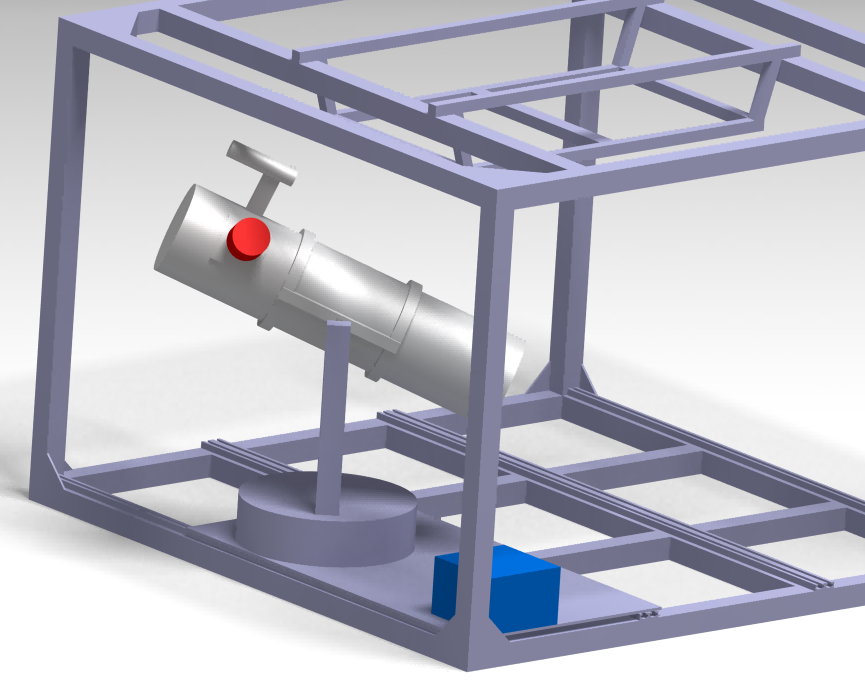
\includegraphics[width=0.9\linewidth]{4-experiment-design/img/interfaces/Assembly_3.png}
	\caption{Instrument position on gondola}
	\label{accomrec}
\end{figure}
